\documentclass[12pt]{article}
\usepackage[a4paper,bindingoffset=0.2in,
            left=1in,right=1in,top=1in,bottom=1in,
            footskip=.25in]{geometry}
\title{User Guide}
\author{SDP Group 15-H}
\usepackage{listings}
\usepackage{color}
\usepackage{graphicx}
\usepackage{parskip}
\usepackage{titling}

\graphicspath{ {images/} }

\definecolor{dkgreen}{rgb}{0,0.6,0}
\definecolor{gray}{rgb}{0.5,0.5,0.5}
\definecolor{mauve}{rgb}{0.58,0,0.82}

\lstset{frame=tb,
  language=bash,
  aboveskip=3mm,
  belowskip=3mm,
  showstringspaces=false,
  columns=flexible,
  basicstyle={\small\ttfamily},
  numbers=none,
  numberstyle=\tiny\color{gray},
  keywordstyle=\color{blue},
  commentstyle=\color{dkgreen},
  stringstyle=\color{mauve},
  breaklines=true,
  breakatwhitespace=true,
  tabsize=3
}

\begin{document}

\begin{figure}
    \vspace*{-3em}
    \centering
    
\includegraphics[scale=.18]{logo.png}
\end{figure}

\setlength{\droptitle}{-4em}
\maketitle

\section{Installation}

\subsection{Cloning the repository and setting up}

To clone the repository, execute in terminal:
\begin{lstlisting}
$ git clone https://github.com/julijonas/venus.git
\end{lstlisting}

Then create a Python virtual environment and install the libraries:
\begin{lstlisting}
$ cd venus
$ virtualenv env
$ source env/bin/activate
$ pip install -r requirements.txt
\end{lstlisting}

To open the Arduino IDE, execute:
\begin{lstlisting}
$ arduino
\end{lstlisting}

You'll need to add three libraries which can be found under \texttt{arduino/} in the project directory: \textit{ArduinoSerialCommand}, \textit{SDPArduino}, \textit{SimpleTimer}. In order to add a library, go to:
\begin{lstlisting}
Sketch -> Import Library... -> Add Library... and choose the library folder you want to import.
\end{lstlisting}

\section{Overview of the robot}

At the current stage, our robot, Venus, can move and kick. It moves because it
has its wheels connected to the NXT motors and we can send commands that power
some of those motors on and off depending which action we want the robot to
perform. The kicker is also connected to another NXT motor, which allows us to
control the power of the kick.

\subsection{Use}

In order to turn the robot on, connect the battery pack to the power board.
In order to swap the batteries, take them out, put them to charge and insert
the new batteries into the battery pack. Easy!

\section{Running instructions}

(To be changed after the first milestone)
\bigskip

Run the command in the terminal from the project root directory:
\begin{lstlisting}
source env/bin/activate
\end{lstlisting}
Then, in order to send commands the robot:
\begin{lstlisting}
python control/control.py
\end{lstlisting}
After that you should be able to send commands to the robot (make sure the RF stick is plugged in).
\bigskip

\textbf{NB} In case you make changes to Arduino code, you should upload your changes to the board!
\bigskip

The list of possible commands is below:
\bigskip
\begin{itemize}
\item For moving to the target in the milestone 1, there is a command 'move'.
\bigskip

At the beggining the robot turns 90 degrees to the right (if "distance1" parameter is positive the robot will move to the forwards, if negative backwards). After covering the first distance it turns 90 degrees so that it faces the same way as at the start. The "degrees" parameter is amount of degrees the robot turns (positive - clockwise, negative - anticlockwise)
\bigskip

\begin{figure}
    \centering
    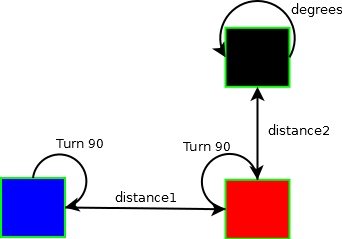
\includegraphics{Diagram1}
\end{figure}

\begin{lstlisting}
move <distance1> <distance2> <degrees>
\end{lstlisting}
\newpage

\item To transfer a file through RF link to I2C port as specified in the milestone:
\begin{lstlisting}
transfer <filename> <frequencyInHz>
\end{lstlisting}

\item To kick the ball a distance specified in the milestone:
\begin{lstlisting}
kick [50|100|150]
\end{lstlisting}

\item To move forward and turn (negative values will change the direction):
\begin{lstlisting}
f <distance>
c <degrees>
\end{lstlisting}

\item To engage the grabber:
\begin{lstlisting}
g
\end{lstlisting}

\item To release the grabber and kick simultaneously:
\begin{lstlisting}
x <kickStrength>
\end{lstlisting}

\item To stop all the motors:
\begin{lstlisting}
s
\end{lstlisting}

\end{itemize}

\section{Troubleshooting guide}
\textbf{Problem 1} When trying to upload the code to the Arduino board, you get the error message below.
\begin{lstlisting}
processing.app.SerialNotFoundException: Serial port '<port>' not found. Did you select the right one from the Tools > Serial Port menu?
\end{lstlisting}

\bigskip

\textbf{Solution}  It can't detect the Arduino board. Make sure it's connected to the computer through the RF stick or the cable. If it is, disconnect and connect again, or power the board off and on again. The Arduino IDE is only able to program the Arduino when the serial interface of the RF stick or Arduino itself is registered as \texttt{/dev/ttyACM0} on the PC, that is, zeroth device. Also, make sure you are not running 'python control/control.py' or have not opened the serial interface any other way when you're uploading the changes.
\bigskip

\textbf{Problem 2} When sending commands the robot doesn't do anything and you're sure it should move.
\bigskip

\textbf{Solution} Power the Arduino board off and on again.


\end{document}